\chapter{Introdución}
\label{chap:introducion}


\section{Motivación}
\lettrine{A}{ctualmente} podemos ver durante nuestro día a día cómo nuestra vida va cada vez más unida al uso de las redes sociales (Figura \ref{evorss}): subimos nuestras fotos, comentamos las de otros, escribimos críticas de artículos que hemos adquirido, escribimos nuestros pensamientos sobre situaciones de actualidad, etc. Aprovechando esta situación vemos que para el mundo empresarial resulta muy interesante el conocer la opinión que los usuarios tienen sobre los productos ofrecidos, o sobre la entidad misma.

\begin{figure}[!ht]
	\centering
	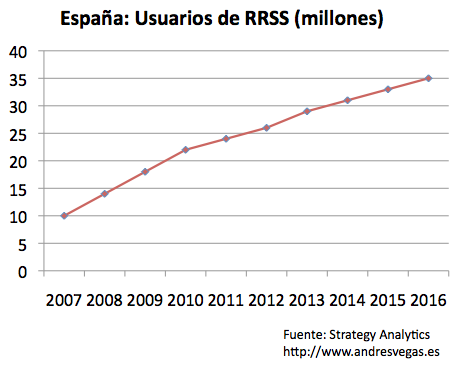
\includegraphics[width=0.75\textwidth]{imaxes/evorss.png}
	\caption{Evolución del uso de las redes sociales}
	\label{evorss}
\end{figure}

Este auge de las redes sociales no solo despierta la curiosidad de los empresarios, sino que también, y de forma muy ligada al interés económico inherente, nos permite disponer de un corpus muy extenso de textos que nos servirán como punto de partida para la construcción de un sistema clasificador.

Además de esto, cabe destacar el gran avance tecnológico realizado en los últimos años, permitiéndonos tener ordenadores cada vez más potentes, con unas capacidades de procesamiento tanto de CPU como de GPU altísimas y gracias a ello realizar entrenamientos con topologías mucho más complejas en un rango de tiempo menor. Es por esto que una de las ramas que hemos investigado para procurar una mejora del resultado final es una aproximación a las redes neuronales, las cuales se entrenan aprovechando la potencia de la GPU.

Hemos visto en este tipo de sistemas una oportunidad de negocio, ofreciendo al cliente ampliar su plataforma implementando un sistema de ranking automático de la lista de resultados mediante un pesado de la polaridad de las opiniones que los usuarios realizan sobre cada uno de los productos. De esta forma los usuarios podrán agilizar sus búsquedas, encontrando en los primeros lugares los elementos más relevantes, y el cliente podría realizar estudios sobre la aceptación de los mismos en el mercado.

\section{Objetivos}

El objetivo de esta investigación es el de analizar y comparar distintos modelos de clasificación de polaridades de textos utilizando procesamiento de lenguaje natural, para posteriormente utilizar estos modelos en la clasificación de comentarios realizados en una web de materiales de construcción.

Además se implementarán los módulos necesarios en una aplicación web para facilitar al usuario la publicación de estos comentarios.

\subsection{Análisis de sentimientos}

La tarea consiste en buscar una serie de características en el texto, en este caso comentarios, presumiblemente breves, sobre materiales de construcción, que nos ayude a realizar una clasificación de los mismos dividiéndolos en distintas clases.

Esta tarea es conocida como Análisis de Sentimiento (Das y Chen \cite{Das}, Tong \cite{Tong}, Turney \cite{Turney}, Pang et al. \cite{Pang}), Extracción de opiniones, Minería de Opiniones (introducido por Dave et al. \cite{Dave}), Minería de sentimiento o Análisis Subjetivo.

El ámbito de clasificación de esta tarea suele ser el siguiente:
\begin{itemize}
	\item Binario: El resultado se divide en dos clases bien diferenciadas (Opinión positiva y opinión negativa)
	\item Multiclase: El resultado se divide en 5 clases (Muy negativa, negativa, neutra, positiva, muy positiva)
	\item Tri-clase: El resultado se divide en 3 clases (Negativa, neutra y positiva)
\end{itemize}

Es de esperar que a mayor número de clases el problema se haga más complicado. Dado el dominio textual de la tarea es más difícil encontrar las diferencias entre un texto muy negativo y uno negativo que entre una opinión negativa y otra positiva.

Esta tarea suele resultar difícil incluso para humanos, ya que la valoración está fuertemente influenciada por valores subjetivos de cada observador. Por ejemplo la frase \emph{No me ha gustado la calidad del producto} podría ser considerada negativa por un observador imparcial y muy negativa por la persona responsable de la calidad de dicho producto.

El punto principal de la tarea es la extracción de características clave del texto que ayuden a separar y clasificar los textos en clases. En este área encontramos 2 aproximaciones principales:

\begin{itemize}
	\item Bag of words (BOW): Es el modelo más simple, se compone un vector de características en el que cada elemento se corresponde a una palabra del dominio, y su valor será o bien el número de ocurrencias en el texto o bien un valor estadístico que refleje la relación de la palabra con su contexto, como por ejemplo el valor de tf-idf.
	\item Word Embeddings (WE): Es un vector compuesto mediante un entrenamiento en una red neuronal que recibe como entrada un conjunto grande de textos e intenta aprender las relaciones de similitud entre las palabras que lo componen, dando como resultado para cada palabra un vector de dígitos reales de una longitud determinada. Gracias a este tipo de datos es posible buscar relaciones de similitud, o incluso operaciones de adición y sustracción entre los vectores que representan las palabras, dando como resultado otra palabra:
	\subitem Vector(Rey) - Vector(Hombre) + Vector(Mujer)  = Vector(Reina)
\end{itemize}


\subsection{Servicio web}
Pretendemos poner a disposición del usuario una web para realizar una búsqueda semántica de los productos, que además les ofrecerá un servicio de comentarios con las siguientes funcionalidades:

\begin{itemize}
	\item Añadir comentarios: Los usuarios podrán añadir nuevos comentarios tanto si están registrados como si son usuarios anónimos.
	\item Editar comentarios: Los usuarios registrados podrán editar sus comentarios.
	\item Borrar comentarios: Los usuarios registrados podrán eliminar sus comentarios.
\end{itemize}

Además el objetivo final de este servicio es clasificar los comentarios de manera que este resultado se pueda utilizar en un sistema de ranking de los resultados ofrecidos por el buscador semántico.
